\begin{center}
\section{Methodology}
\label{method}
\end{center}

An organised approach to the evaluation and testing is required to study the proposed algorithms analytically. The Travelling Salesman Problem is a single-objective optimisation problem\cite{Halim2021} with the sole goal of minimising the route cost(Equation\ref{TSPcost}). However, it is not the only metric worth considering when evaluating heuristics, as runtime is a major factor in determining which algorithm to use\cite{rardin2001experimental}. Therefore, the data collection method must remain unbiased for the comparisons to have validity.

Empirical research is a research method that involves observing the direct result of an action and gathering data\cite{patten2016proposing}. The values observed are considered empirical data, which can be quantitatively analysed to aid in decision making and reaching a conclusion\cite{patten2016proposing}. Due to the nature of NP-hard problems, it is improbable\cite{Halim2021} to test heuristics against random exact solutions. Therefore, comparing them to other heuristics is an appropriate approach; this is called blind(statistical) testing\cite{BHATTACHARJEE2022100471}.

\subsection{Empirical Testing}

Using large data collection and data analysis, trends and properties are outlined in the testing, which would otherwise be obscured by randomness\cite{BHATTACHARJEE2022100471}. Much like real-life experiments, the collected data(dependent variable) must have controlled variables and a single independent variable. The independent variable is the algorithm and its unique parameters, thus SLACIH(1) and SLACIH(2) are two different independent variable entries. The control is the identical Travelling Salesman Problem and system properties executed for each algorithm. A set of experiments with the same control variable is referred to as an instance. Generating multiple random instances creates a data table in a process known as Instances vs Algorithm\cite{BHATTACHARJEE2022100471}. In the table, all instances must have the same TSP properties, e.g. problem size and random generation method.

\begin{figure}[!ht]
    \centering
    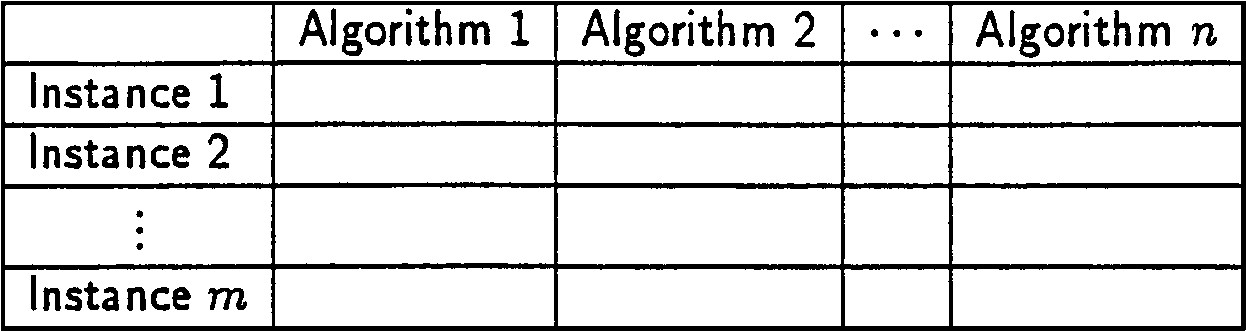
\includegraphics[width=0.7\textwidth]{sections/image/empirical.jpg}
    \caption{Instances Vs Algorithm}
    \cite{rardin2001experimental}
\end{figure}

Once the table has been populated with a sufficient number of instances, to reduce randomness, data analysis can be used to draw conclusions. Statistical properties, such as averages, standard deviation, and inference, are explored as avenues for comparison.

\subsection{TSPLib}

In the research for the Travelling Salesman Problem, there is a library of tests called TSPLib\cite{TSPLIB95}, which contains famous real-world examples and common pitfall problems. It contains 130 problems of varying graph sizes, with the largest having 85,900 nodes. All have been solved with an exact solution by the Concorde TSP Solver(Section\ref{Concorde}), making TSPLib a suitable library for benchmarking heuristics against the global optimal\cite{TSPLibBench}. TSPLib is also useful as a ground truth for comparing research papers due to its ubiquity as a benchmark.

\begin{figure}[H]
    \centering
    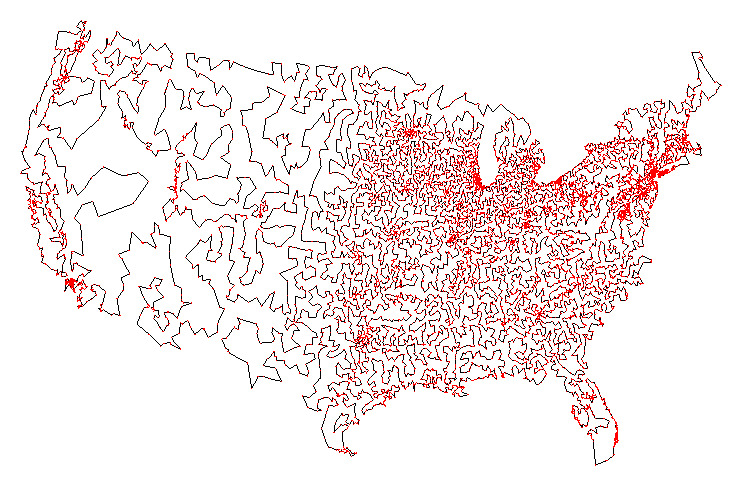
\includegraphics[width=0.7\textwidth]{sections/image/usa13509.sol-ezgif.com-gif-to-jpg-converter.jpg}
    \caption{TSPLib: USA13509} 
    \cite{chvatal2001tsp}
\end{figure}

As the problem solutions vary in cost, taking the difference from the optimal solution as a percentage(Equation\ref{psolution}) allows for calculating the average performance of a heuristic across the entire TSPLib(Equation\ref{ptsplib}). This normalisation allows for each problem to contribute evenly to a heuristic score.

\begin{equation}
    p_{solution}=\frac{solution_{heuristic}-solution_{optimal}}{solution_{optimal}}
    \label{psolution}
\end{equation}

\begin{equation}
    p_{TSPLib}=\frac{\sum{p_{solution}}}{|p_{solution}|}
    \label{ptsplib}
\end{equation}